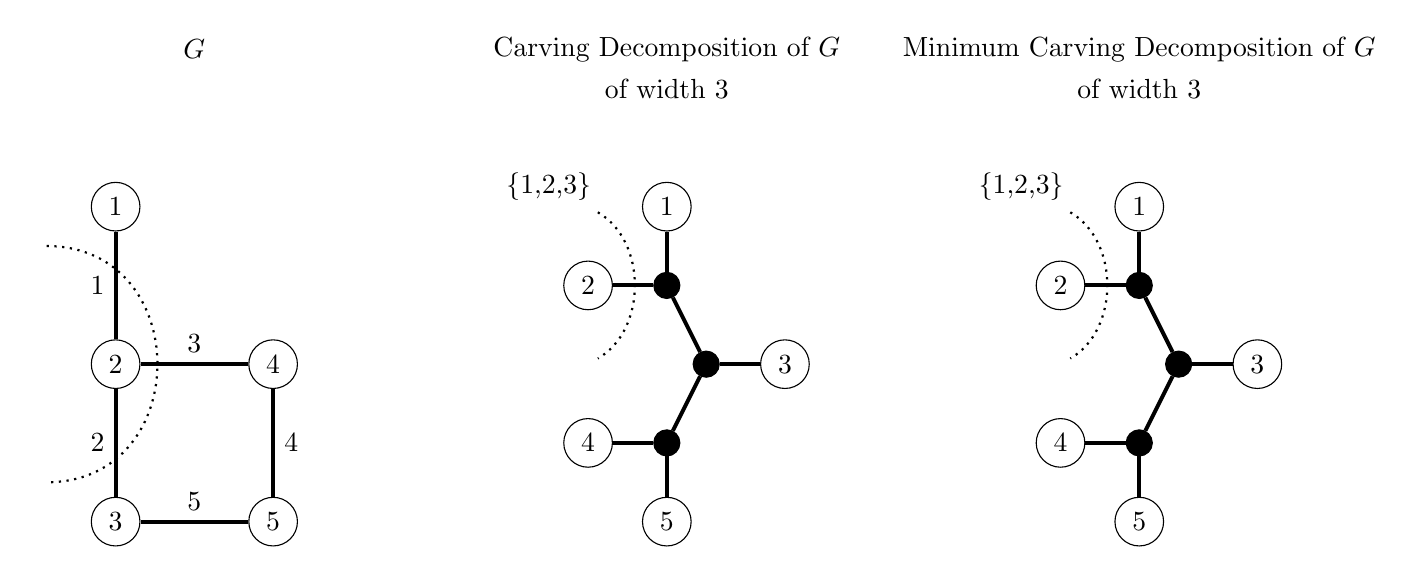
\begin{tikzpicture}
	\begin{scope}[xshift=0cm, yshift=0cm]
		\node (G) at (1, 6) {$G$};

		\node[circle, draw] (a1) at (0, 4) {1};
		\node[circle, draw] (a2) at (0, 2) {2};
		\node[circle, draw] (a3) at (0, 0) {3};
		\node[circle, draw] (a4) at (2, 2) {4};
		\node[circle, draw] (a5) at (2, 0) {5};
	
		% Draw the edges between nodes with labels
		\draw[line width=0.5mm] (a1) -- node[left] {1} (a2);
		\draw[line width=0.5mm] (a2) -- node[left] {2} (a3);
		\draw[line width=0.5mm] (a2) -- node[above] {3} (a4);
		\draw[line width=0.5mm] (a4) -- node[right] {4} (a5);
		\draw[line width=0.5mm] (a3) -- node[above] {5} (a5);

		\node[opacity=0] at (-1, 3.5) (start) {};
		\node[opacity=0] at (-1, 0.5) (end) {};
		\draw[dotted, thick] (start) .. controls +(2,0) and +(2,0) .. (end);
	\end{scope}

	\begin{scope}[xshift=6cm, yshift=0cm]
		\node (G) at (1, 6) {Carving Decomposition of $G$};
		\node (G) at (1, 5.5) {of width 3};

		\node[circle, draw, color=black, fill=white] (b1) at (1, 4) {1};
		\node[circle, draw, color=black, fill=white] (b3) at (0, 3) {2};
		\node[circle, draw, color=black, fill=black] (i1) at (1, 3) {};
		\node[circle, draw, color=black, fill=black] (i2) at (1.5, 2) {};
		\node[circle, draw, color=black, fill=black] (i3) at (1, 1) {};
		\node[circle, draw, color=black, fill=white] (b2) at (2.5, 2) {3};
		\node[circle, draw, color=black, fill=white] (b4) at (0, 1) {4};
		\node[circle, draw, color=black, fill=white] (b5) at (1, 0) {5};
	
		% Draw the edges between nodes with labels
		\draw[line width=0.5mm, color=black] (b1) -- (i1);
		\draw[line width=0.5mm, color=black] (b3) -- (i1);
		\draw[line width=0.5mm, color=black] (i1) -- (i2);
		\draw[line width=0.5mm, color=black] (b2) -- (i2);
		\draw[line width=0.5mm, color=black] (i2) -- (i3);
		\draw[line width=0.5mm, color=black] (i3) -- (b4);
		\draw[line width=0.5mm, color=black] (i3) -- (b5);

		\node (G) at (-0.5, 4.25) {\{1,2,3\}};
		
		\node[opacity=0] at (0,4) (start) {};
		\node[opacity=0] at (0,2) (end) {};
		\draw[dotted, thick] (start) to[bend left=60] (end);
	\end{scope}

	\begin{scope}[xshift=12cm, yshift=0cm]
		\node (G) at (1, 6) {Minimum Carving Decomposition of $G$};
		\node (G) at (1, 5.5) { of width 3};

		\node[circle, draw, color=black, fill=white] (b1) at (1, 4) {1};
		\node[circle, draw, color=black, fill=white] (b3) at (0, 3) {2};
		\node[circle, draw, color=black, fill=black] (i1) at (1, 3) {};
		\node[circle, draw, color=black, fill=black] (i2) at (1.5, 2) {};
		\node[circle, draw, color=black, fill=black] (i3) at (1, 1) {};
		\node[circle, draw, color=black, fill=white] (b2) at (2.5, 2) {3};
		\node[circle, draw, color=black, fill=white] (b4) at (0, 1) {4};
		\node[circle, draw, color=black, fill=white] (b5) at (1, 0) {5};
	
		% Draw the edges between nodes with labels
		\draw[line width=0.5mm, color=black] (b1) -- (i1);
		\draw[line width=0.5mm, color=black] (b3) -- (i1);
		\draw[line width=0.5mm, color=black] (i1) -- (i2);
		\draw[line width=0.5mm, color=black] (b2) -- (i2);
		\draw[line width=0.5mm, color=black] (i2) -- (i3);
		\draw[line width=0.5mm, color=black] (i3) -- (b4);
		\draw[line width=0.5mm, color=black] (i3) -- (b5);

		\node (G) at (-0.5, 4.25) {\{1,2,3\}};

		\node[opacity=0] at (0,4) (start) {};
		\node[opacity=0] at (0,2) (end) {};
		\draw[dotted, thick] (start) to[bend left=60] (end);
	\end{scope}
\end{tikzpicture}
